% predicate-read.tex

\documentclass[tikz, border=2pt]{standalone}

\usepackage[dvipsnames]{xcolor}

\begin{document}
  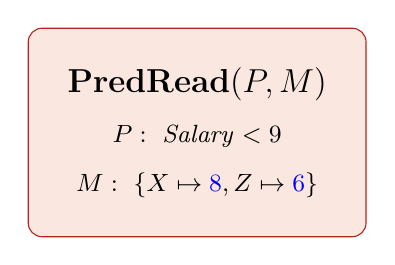
\begin{tikzpicture}[
      font = \large,
      op/.style={
        draw = BrickRed,
        rounded corners = 5pt,
        fill = BrickRed!8,
        inner sep = 5mm,
        align = center,
      },
    ]
    \node[op] {\textbf{PredRead}$(P,M)$\\[.35em]
      \small $P:\ \mathit{Salary} < 9$\\[.30em]
      \small $M:\ \{X \mapsto \textcolor{blue}{8},
        Z \mapsto \textcolor{blue}{6}\}$};
  \end{tikzpicture}
\end{document}